% 第5章第1节：点值与再生核（点值泛函与再生关系、再生核的性质）。

\section{点值与再生核}
\label{sec:rkhs-point-evaluation}

本节固定一个由真实函数组成的Hilbert空间，要求每个点的取值都连续地依赖于函数。第~\ref{sec:lfo-point-evaluation}节已经把点值读取的良定义与有界性分开讨论；这里把两项要求同时作为空间的前提，再用第~\ref{sec:lfo-riesz}节的Riesz表示把每个点的读取写成内积。由此得到的二元函数称为再生核。第~\ref{sec:rkhs-kernel-properties}节再从核本身读出点值的强弱、核矩阵的符号，以及读数随位置变化的方式。

\subsection{点值泛函与再生关系}
\label{sec:rkhs-reproducing}
\label{subsubsec:point-evaluation}

\paragraph{点值读取的两项要求}

回顾第~\ref{sec:lfo-point-evaluation}节的两个反例。在Lebesgue测度下，$L^2[0,1]$的元素是几乎处处相等的函数类，零函数与只在$x=1/2$处取$1$的函数属于同一类，却给出不同的点值，所以“取$1/2$处的值”在$L^2$上没有良定义。即使只考虑连续函数，尖峰$f_n(t)=\max(1-nt,0)$满足$\|f_n\|_{L^2}^2=1/(3n)$而$f_n(0)=1$，比值$f_n(0)/\|f_n\|_{L^2}=\sqrt{3n}$没有上界，原点的读取不受$L^2$范数控制。

这两个反例说明，点值要成为可靠的信息，空间必须同时满足两条：元素是真正的函数，每个$f(x)$都有确定的数值；并且对每个固定的$x$，读取$f\mapsto f(x)$是有界线性泛函。第一条由空间的选取保证，第二条则依赖空间所带的范数。下面的例子同时满足两条，它会在本章反复出现。

\paragraph{一个满足两项要求的空间}

令$H_{\min}$为$[0,1]$上满足$f(0)=0$、几乎处处导数$f'\in L^2(0,1)$的绝对连续函数全体，内积取
\[
\langle f,g\rangle_{H_{\min}}=\int_0^1f'(t)g'(t)\,\mathrm dt .
\]
绝对连续保证$f(x)=\int_0^xf'(t)\,\mathrm dt$，所以映射$f\mapsto f'$把$H_{\min}$一一地映到$L^2(0,1)$上，逆映射是$g\mapsto\int_0^{\,\cdot}g$，并且保持内积。由此，$\langle f,f\rangle=0$迫使$f'=0$几乎处处，再由$f(0)=0$得$f=0$；$L^2(0,1)$的完备性也随这个等距对应传到$H_{\min}$。这些函数正是第~\ref{sec:sob-absolute-continuity}节中$H^1(0,1)$元素的连续代表里左端取零的那一部分。

在$H_{\min}$中读取一点的值，只需对导数作Cauchy--Schwarz估计：
\begin{equation}
|f(x)|=\Bigl|\int_0^x f'(t)\,\mathrm dt\Bigr|
\le\Bigl(\int_0^x1\,\mathrm dt\Bigr)^{1/2}\|f'\|_{L^2}
=\sqrt x\,\|f\|_{H_{\min}} .
\label{eq:rkhs-hmin-point-bound}
\end{equation}
因此每个点的读取都有界，常数$\sqrt x$随位置变化，在整个区间上不超过$1$。这与第~\ref{sec:sob-embedding}节一维Sobolev函数的点值估计是同一个机制：导数的平方积分控制了函数沿路径的累计变化，再由左端的固定值得到点值。

\paragraph{再生核Hilbert空间的定义}

把上述两项要求抽象出来，就得到本章的研究对象。

\begin{definition}[再生核Hilbert空间]
\label{def:rkhs-rkhs}
设$X$是非空集合，$H$是由函数$f:X\to\mathbb R$组成的实Hilbert空间，其加法与数乘按逐点方式定义。若对每个$x\in X$，\term{点值泛函}（evaluation functional）$L_x:H\to\mathbb R$，$L_x(f)=f(x)$都是有界线性泛函，则称$H$为\term{再生核Hilbert空间}（reproducing kernel Hilbert space，RKHS）。
\end{definition}

定义中逐点运算这一条不能省略：它保证$H$的零元就是处处为零的函数，从而“两个元素相等”与“两个函数在每一点取值相同”是同一件事。$L^2$的元素不是这样的函数，所以它不在定义的讨论范围之内，这与它的点值读取没有良定义是一致的。

对每个$x$，$L_x$有界且$H$是Hilbert空间，第~\ref{sec:lfo-riesz}节的Riesz表示给出唯一的$K_x\in H$，使得
\begin{equation}
f(x)=\langle f,K_x\rangle_H\qquad(f\in H),
\label{eq:rkhs-reproducing}
\end{equation}
并且$\|L_x\|=\|K_x\|_H$。$K_x$本身也是$X$上的函数。定义二元函数
\begin{equation}
K(z,x)=K_x(z)=\langle K_x,K_z\rangle_H\qquad(x,z\in X),
\label{eq:rkhs-kernel-definition}
\end{equation}
其中第二个等号是对$f=K_x$在点$z$处使用式~\eqref{eq:rkhs-reproducing}。称$K$为$H$的\term{再生核}（reproducing kernel），称$K_x=K(\cdot,x)$为核在$x$处的\term{核截面}（kernel section）。式~\eqref{eq:rkhs-reproducing}称为\term{再生性质}（reproducing property）：在$x$处读取$f$，等于拿$f$与固定函数$K_x$作内积；把$f$换成$K_z$，读出的又是核本身的值，“再生”一词即由此而来。

\paragraph{仿射函数空间中的核验}

最小的非平凡例子是仿射函数空间
\[
H_{\mathrm{aff}}=\{f(t)=a+bt:\ a,b\in\mathbb R\},\qquad
\langle a+bt,\ a'+b't\rangle=aa'+bb' ,
\]
输入集取$X=\mathbb R$。这个内积就是系数向量的欧氏内积，所以$H_{\mathrm{aff}}$是二维Hilbert空间。我们来找$K_x$：它应是某个仿射函数$c+dt$，满足$\langle a+bt,c+dt\rangle=ac+bd=a+bx$对一切$a,b$成立，于是$c=1$、$d=x$，即
\[
K_x(t)=1+xt,\qquad K(t,x)=1+xt .
\]
逐项核对再生性质：$\langle a+bt,K_x\rangle=a\cdot1+b\cdot x=f(x)$。

图~\ref{fig:rkhs-reproducing-geometry}把这个计算画在系数平面上。由于系数平面与$H_{\mathrm{aff}}$等距，每个核截面$K_x$对应向量$(1,x)$，它们全都落在竖直直线$a=1$上。读取$f=1+t$在$x=1/2$处的值，就是计算$(1,1)$与$(1,1/2)$的内积$1.5$；而$K_{-1}=(1,-1)$与$(1,1)$正交，对应$f(-1)=0$。一个函数在某点取零，几何上就是它与该点的核截面垂直。

\begin{figure}[!htb]
  \centering
  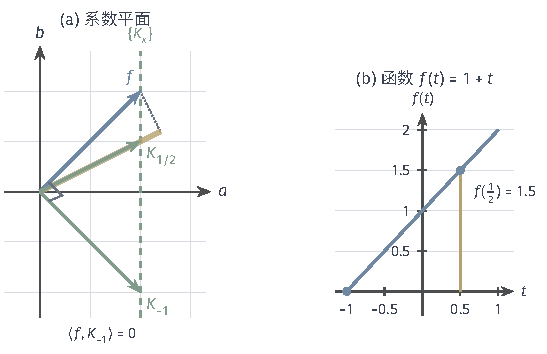
\includegraphics[width=92.7mm]{figures/02-abstract-mathematics/03-function-spaces/tikz/c5-reproducing-geometry/figure.pdf}
  \caption{仿射函数空间中再生性质的几何。(a)~系数平面$(a,b)$与空间等距；$f=1+t$对应$(1,1)$，核截面$K_x=1+xt$对应$(1,x)$，都落在虚线$a=1$上。黄色线段是$f$在$K_{1/2}$方向上的投影，其长度乘以$\|K_{1/2}\|$等于$f(1/2)=1.5$；$K_{-1}$与$f$垂直。(b)~同一函数的图像，标出$t=1/2$处的读数$1.5$与$t=-1$处的零点。}
  \label{fig:rkhs-reproducing-geometry}
\end{figure}

\paragraph{最小值核}

在$H_{\min}$中，核截面同样可以直接猜出来。式~\eqref{eq:rkhs-hmin-point-bound}的推导把$f(x)$写成了$\int_0^1f'(t)\mathbf 1_{[0,x]}(t)\,\mathrm dt$，所以只需找一个导数为$\mathbf 1_{[0,x]}$、左端取零的函数，它就是
\[
K_x(t)=\min(t,x),\qquad K(t,x)=\min(t,x)\qquad(t,x\in[0,1]).
\]
$K_x$在$[0,x]$上斜率为$1$，在$[x,1]$上保持常数$x$，确实属于$H_{\min}$，并且$\langle f,K_x\rangle_{H_{\min}}=\int_0^xf'(t)\,\mathrm dt=f(x)$。称$K(x,z)=\min(x,z)$为$[0,1]$上的\term{最小值核}（minimum kernel）。它在概率论中是标准Brown运动的协方差，但这里只把它当作一个确定的二元函数使用。

\paragraph{逐点常数与统一常数}

定义只要求每个$L_x$有界，有界常数$\|L_x\|$允许随$x$变化。在$H_{\mathrm{aff}}$中，$\|L_x\|=\|K_x\|=\sqrt{1+x^2}$。所以单位球中的函数在$x$处的取值恰好填满区间$[-\sqrt{1+x^2},\sqrt{1+x^2}]$：上界由Cauchy--Schwarz不等式给出，取$f=K_x/\|K_x\|$即可达到。

图~\ref{fig:rkhs-pointwise-envelope}画出这条包络和几条单位范数函数$\cos\theta+t\sin\theta$。每条函数在$t=\tan\theta$处与上包络相切，这正是它与$K_t$同向的位置。在整条实轴上，包络随$|t|$无限增长，不存在统一的常数$C$使$|f(t)|\le C\|f\|$对一切$t$成立；若把输入集限制为$[-1,1]$，统一常数就是$\sqrt2$。一般地，只有当$\sup_{x\in X}K(x,x)<\infty$时，核范数才能统一控制全域的点值误差：
\[
\sup_{x\in X}|f(x)-g(x)|\le\Bigl(\sup_{x\in X}\sqrt{K(x,x)}\Bigr)\,\|f-g\|_H .
\]
对$H_{\min}$，由式~\eqref{eq:rkhs-hmin-point-bound}，统一常数是$1$。

\begin{figure}[!htb]
  \centering
  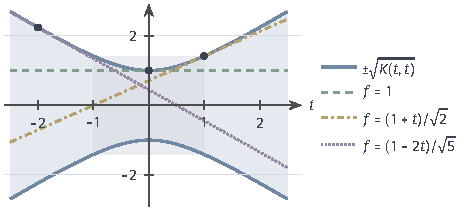
\includegraphics[width=79.6mm]{figures/02-abstract-mathematics/03-function-spaces/tikz/c5-pointwise-envelope/figure.pdf}
  \caption{仿射函数空间单位球在各点的取值范围。浅蓝区域介于$\pm\sqrt{K(t,t)}=\pm\sqrt{1+t^2}$之间；三条虚线是单位范数函数，各自在黑点处与上包络相切。灰色区域标出$[-1,1]$，其中包络的最大值为$\sqrt2$。包络在整条实轴上无界，说明逐点有界不等于统一有界。}
  \label{fig:rkhs-pointwise-envelope}
\end{figure}

\paragraph{离散空间也是RKHS}

再看一个点值有界、函数却毫无连续性的例子。对任意非空集合$X$，令$\ell^2(X)$为满足$\sum_{x\in X}f(x)^2<\infty$的函数全体（求和对至多可数个非零项进行），内积为$\sum_xf(x)g(x)$。显然$|f(x)|\le\|f\|$，所以它是RKHS，其核截面是单点示性函数$K_x=\mathbf 1_{\{x\}}$，再生核是$K(x,z)=1$（$x=z$）或$0$（$x\neq z$）。即使$X=[0,1]$，这个空间中的函数也可以在每点任意跳动。可见点值有界只是对每个固定位置的要求，函数是否随位置连续，需要核提供更多信息。

\subsection{再生核的性质}
\label{sec:rkhs-kernel-properties}

上一小节从空间得到了核。核是一个具体的二元函数，下面看它从三个方面记录空间的信息：每点读取的强弱、任意有限点组上核值矩阵的符号，以及读数随位置的变化。

\paragraph{对称性、半正定性与点值范数}

由定义式~\eqref{eq:rkhs-kernel-definition}，核值是两个核截面的内积，因此内积的性质直接转化为核的性质。

\begin{theorem}[再生核的基本性质]
\label{thm:rkhs-kernel-properties}
设$H$是$X$上的RKHS，$K$为其再生核。则：
\begin{enumerate}
\item 对称性：$K(x,z)=K(z,x)$对一切$x,z\in X$成立；
\item 半正定性：对任意$n\ge1$、任意点$x_1,\ldots,x_n\in X$与实数$a_1,\ldots,a_n$，
\[
\sum_{i,j=1}^na_ia_jK(x_i,x_j)=\Bigl\|\sum_{i=1}^na_iK_{x_i}\Bigr\|_H^2\ge0 ;
\]
\item 点值范数：$\|L_x\|=\|K_x\|_H=\sqrt{K(x,x)}$；并且对任意$x,z\in X$，$|K(x,z)|\le\sqrt{K(x,x)K(z,z)}$。
\end{enumerate}
\end{theorem}

\begin{proof}
由式~\eqref{eq:rkhs-kernel-definition}，$K(x,z)=\langle K_z,K_x\rangle$，实内积的对称性给出第1条。把$\bigl\|\sum_ia_iK_{x_i}\bigr\|^2$按双线性展开为$\sum_{i,j}a_ia_j\langle K_{x_i},K_{x_j}\rangle$，再用$\langle K_{x_i},K_{x_j}\rangle=K(x_j,x_i)=K(x_i,x_j)$，得到第2条。Riesz表示给出$\|L_x\|=\|K_x\|$，而$\|K_x\|^2=\langle K_x,K_x\rangle=K(x,x)$。最后，$|K(x,z)|=|\langle K_z,K_x\rangle|\le\|K_z\|\|K_x\|$。
\end{proof}

第2条中的矩阵$\bm G=[K(x_i,x_j)]_{i,j=1}^n$称为点组$x_1,\ldots,x_n$上的\term{Gram矩阵}或\term{核矩阵}（kernel matrix）。第2条说的就是：每个Gram矩阵都是对称半正定矩阵。这一性质不依赖于空间，只依赖于核，因此可以单独作为对二元函数的要求。

\begin{definition}[半正定核与严格正定核]
\label{def:rkhs-psd-kernel}
设$X$是非空集合。若函数$K:X\times X\to\mathbb R$对称，且对任意有限点组，其Gram矩阵都半正定，则称$K$为$X$上的半正定核，文献中也常称为\term{正定核}（positive definite kernel）。若对任意互异点$x_1,\ldots,x_n$及任意不全为零的实数$a_1,\ldots,a_n$都有$\sum_{i,j}a_ia_jK(x_i,x_j)>0$，即互异点上的Gram矩阵都可逆，则称$K$为\term{严格正定核}（strictly positive definite kernel）。
\end{definition}

“正定核”这个通行名称容易引起误解：它允许Gram矩阵奇异。本书在需要强调时写“半正定核”，与严格正定的情形区分。

\paragraph{仿射核的奇异Gram矩阵}

仿射核说明这种区分是必要的。取三个点$-1,0,1$，Gram矩阵与一个零向量为
\[
\bm G=\begin{bmatrix}2&1&0\\1&1&1\\0&1&2\end{bmatrix},\qquad
\bm G\begin{bmatrix}1\\-2\\1\end{bmatrix}=\bm 0 .
\]
对应的函数组合$K_{-1}-2K_0+K_1=(1-t)-2+(1+t)$恰好是零函数。原因很直接：$H_{\mathrm{aff}}$只有二维，任意三个核截面必然线性相关。图~\ref{fig:rkhs-gram-matrices}对五个点比较了两种核：高斯核$K(x,z)=\exp\bigl(-(x-z)^2/(2\sigma^2)\bigr)$（$\sigma=0.5$）的Gram矩阵五个特征值都为正，仿射核的Gram矩阵则只有两个正特征值$5$与$2.5$，其余三个为零。两者都是半正定核，只有前者在这个点组上可逆。

\begin{figure}[!htb]
  \centering
  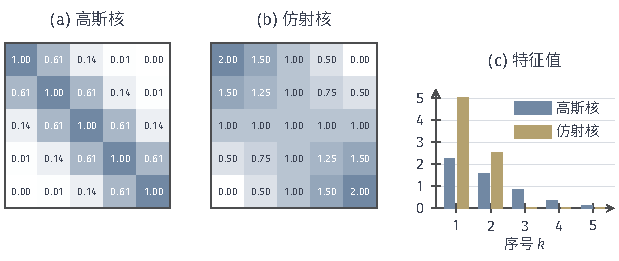
\includegraphics[width=104.8mm]{figures/02-abstract-mathematics/03-function-spaces/tikz/c5-gram-matrices/figure.pdf}
  \caption{点组$x=-1,-0.5,0,0.5,1$上的Gram矩阵。(a)~高斯核（$\sigma=0.5$），颜色越深核值越大，数字保留两位小数（右上角的$0.00$实为$e^{-8}\approx0.0003$）；(b)~仿射核$1+xz$；(c)~两个矩阵的特征值。高斯核的特征值$2.217,1.531,0.820,0.333,0.099$全为正；仿射核只有$5$与$2.5$两个正特征值，其余为零。两种核都半正定，只有前者的矩阵可逆。}
  \label{fig:rkhs-gram-matrices}
\end{figure}

高斯核在任意有限个互异实数上都给出可逆Gram矩阵，即它是严格正定核。这一结论的证明需要Fourier变换，这里不展开；本章后面用到高斯核时，只在具体计算中检查相应矩阵的可逆性。严格正定性与半正定性是两项不同的要求：半正定性可由第~\ref{sec:rkhs-kernel-operations}节的运算规则逐步验证，严格正定性则须对互异点组另行判断。

\paragraph{核截面的形状}

核截面$K_x$是$H$中的元素，所以它的形状直接展示了空间中函数的样子。图~\ref{fig:rkhs-kernel-sections}画出三种核在$[-1,1]$上的截面。高斯核的截面是以$x$为中心的钟形，离$x$越远取值越小；仿射核的截面是过点$(0,1)$的直线；二次多项式核$(1+xt)^2$的截面是抛物线。后两种核的截面都只在有限维函数族中变化，它们张成的空间分别是仿射函数与至多二次的多项式；高斯核截面则彼此不在任何有限维子空间中，这与它的严格正定性相符。

\begin{figure}[!htb]
  \centering
  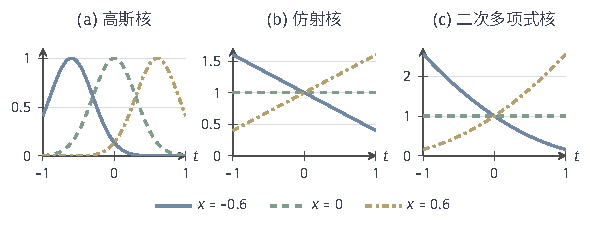
\includegraphics[width=99.9mm]{figures/02-abstract-mathematics/03-function-spaces/tikz/c5-kernel-sections/figure.pdf}
  \caption{三种核在$[-1,1]$上的核截面$K_x(t)=K(t,x)$，$x=-0.6,0,0.6$。(a)~高斯核（$\sigma=0.3$），截面是以$x$为中心的钟形；(b)~仿射核$1+xt$，截面是直线；(c)~二次多项式核$(1+xt)^2$，截面是抛物线。核截面是空间中的元素，其形状展示了空间所含函数的类型。}
  \label{fig:rkhs-kernel-sections}
\end{figure}

\paragraph{位置变化与核截面的距离}

到目前为止，每个点的读取是分开讨论的。现在固定函数$f$，只移动读取位置。由再生性质，
\[
f(x)-f(z)=\langle f,K_x-K_z\rangle_H ,
\]
所以
\begin{equation}
\begin{gathered}
|f(x)-f(z)|\le\|f\|_H\,\|K_x-K_z\|_H,\\
\|K_x-K_z\|_H^2=K(x,x)+K(z,z)-2K(x,z) .
\end{gathered}
\label{eq:rkhs-position-bound}
\end{equation}
第二个等式由展开$\langle K_x-K_z,K_x-K_z\rangle$并使用式~\eqref{eq:rkhs-kernel-definition}得到。式~\eqref{eq:rkhs-position-bound}把位置的变化转化为两个核截面在$H$中的距离，而这个距离只用核的三个值就能算出。

对三个例子分别计算这个距离。高斯核满足$K(x,x)=1$，于是$\|K_x-K_z\|^2=2-2e^{-d^2/(2\sigma^2)}$，其中$d=|x-z|$；由$1-e^{-u}\le u$得$\|K_x-K_z\|\le d/\sigma$，所以单位范数函数满足$|f(x)-f(z)|\le|x-z|/\sigma$。最小值核满足$\|K_x-K_z\|^2=x+z-2\min(x,z)=|x-z|$，于是$|f(x)-f(z)|\le\|f\|_{H_{\min}}|x-z|^{1/2}$，这正是一维Sobolev函数的$1/2$阶Hölder估计。离散空间$\ell^2(X)$的核在$x\neq z$时给出$\|K_x-K_z\|=\sqrt2$，距离不随$|x-z|$缩小。图~\ref{fig:rkhs-section-distance}把这些曲线画在一起：前两类核截面随位置连续移动，最后一类在每一点都跳开。

\begin{figure}[!htb]
  \centering
  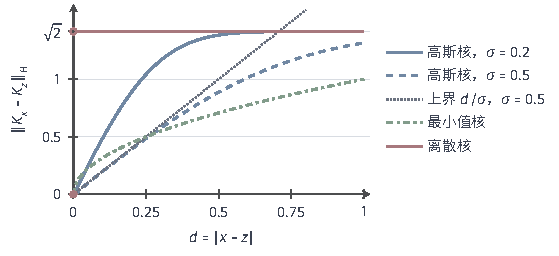
\includegraphics[width=94.7mm]{figures/02-abstract-mathematics/03-function-spaces/tikz/c5-section-distance/figure.pdf}
  \caption{核截面距离$\|K_x-K_z\|_H$随位置差$d=|x-z|$的变化。两条蓝线是高斯核（$\sigma=0.2$与$0.5$），点线是$\sigma=0.5$时的上界$d/\sigma$；绿色点划线是最小值核的$\sqrt d$；红线是离散空间$\ell^2(X)$的核，$d>0$时恒为$\sqrt2$。由式~\eqref{eq:rkhs-position-bound}，这个距离乘以$\|f\|_H$控制了$|f(x)-f(z)|$；前三条曲线在$d\to0$时趋于零，最后一条不然。}
  \label{fig:rkhs-section-distance}
\end{figure}

\paragraph{连续核与函数的连续性}

上述计算可以整理成一条一般结论。

\begin{theorem}[连续核给出连续函数]
\label{thm:rkhs-continuity}
设$X$是度量空间，$H$是$X$上的RKHS，再生核$K$在$X\times X$上连续。则：
\begin{enumerate}
\item 映射$x\mapsto K_x$从$X$到$H$连续，因而每个$f\in H$都是$X$上的连续函数；
\item 若$X$还是紧的，则对任意$R>0$，球$B_R=\{f\in H:\|f\|_H\le R\}$中的函数一致有界且等度连续：对任意$\varepsilon>0$存在$\delta>0$，使得$d(x,z)<\delta$时，对一切$f\in B_R$都有$|f(x)-f(z)|<\varepsilon$。
\end{enumerate}
\end{theorem}

\begin{proof}
当$z\to x$时，$K$的连续性使$K(z,z)\to K(x,x)$、$K(x,z)\to K(x,x)$，由式~\eqref{eq:rkhs-position-bound}的第二个等式得$\|K_x-K_z\|\to0$；再由第一个不等式，$f(z)\to f(x)$。这证明第1条。

若$X$紧，则$X\times X$紧，连续函数$K$一致连续（第~\ref{sec:metric-compact-continuous}节），并且对角线上的$K(x,x)$有最大值$M^2$。一致连续性给出：对任意$\eta>0$存在$\delta>0$，使得$d(x,z)<\delta$时$K(x,x)+K(z,z)-2K(x,z)<\eta$。取$\eta=(\varepsilon/R)^2$，式~\eqref{eq:rkhs-position-bound}便对$B_R$中所有$f$同时给出$|f(x)-f(z)|<\varepsilon$；一致有界性来自$|f(x)|\le M\|f\|\le MR$。
\end{proof}

第2条中的$\delta$只依赖于核与半径$R$，不依赖于球中具体的函数，这是“共同的连续性控制”的含义。第~\ref{sec:apx-arzela-ascoli}节将用这种一致有界、等度连续的性质判断函数族的紧性。还要强调两种稳定性的区别：固定位置时，$|f(x)-g(x)|\le\sqrt{K(x,x)}\|f-g\|_H$描述函数改变引起的读数改变；固定函数时，式~\eqref{eq:rkhs-position-bound}描述位置改变引起的读数改变。离散空间$\ell^2([0,1])$说明前者成立并不蕴含后者。
